\chapter{Analyser}\label{Analyser}

\section{Brugerundersøgelser}
Der er brugt både kvalitative og kvantitative undersøgelser til belysning af projektets problemstillinger. Den kvalitative metode er anvendt til interviews af radiolog Lars Boldvig og afdelingsradiograf Tine Bisgaard for at undersøge praksis ved ultralydsscanninger. Den kvantitative metode er benyttet i sammenhæng med den kvalitative ifm. spørgeskemaundersøgelsen af potentielle patienter. Der blev stillet kvalitative spørgsmål som herefter blev kvantificeret.

\subsection*{Spørgeskemaundersøgelse}
Spørgeskemaundersøgelsen, bestående af et kvalitativt spørgeskema med tre spørgsmål samt spørgsmål om aldersgruppe og køn, er lavet for at undersøge potentielle patienters meninger om at blive undersøgt af en automatiseret robot. Der blev spurgt om tanker angående scanning af en automatiseret robot fremfor en radiolog, samt hvilke problemstillinger og fordele respondenterne ser ved en automatiseret ultralydsscanner. 

Der var i alt 72 respondenter på spørgeskemaet, hvor størstedelen, 87,5\%, af respondenterne var positive over for at blive scannet af en automatisk robot. De sidste 12,5\% var negative eller bekymrede. Respondenterne ser både fordele og ulemper ved scanningerne, som kan læses i bilag \ref{Sporgeskemaundersogelse} Spørgeskemaundersøgelse. Se respondenternes fulde svar i bilag \ref{Patientsvar} Patientsvar. 

Spørgeskemaundersøgelsen blev lavet før projektets problemstilling var færdigdefineret, og derfor falder den lidt ved siden af projektet. Den er dog stadig medtaget i projektet, fordi den kan give en indikation af, hvordan og hvad der skal til, før patienter vil tage imod Automatisk Ultralydsscanner. 

\subsection*{Interview med afdelingsradiograf} 
Aarhus Universitetshospital, Tage-Hansens Gade, blev kontaktet for inspiration og belysning af den daglige praksis på Røntgen- og Skanningsafdeling, samt for at undersøge sundhedsfagliges meninger om Automatisk Ultralydsscanner. Afdelingsradiograf Tine Bisgaard indvilgede i at vise rundt på afdelingen samt svare på spørgsmål om afdelingens dagligdag. 

Tine Bisgaard vurderede mammografi af begge bryster til at vare 5 minutter, mens en ultralydsscanning blev vurderet til at vare omkring 10 minutter, afhængigt af radiologens rutine. Tine Bisgaard mener ikke, at det vil være et problem at benytte en automatisk ultralydsscanner til at udføre scanninger, hvis man blot informerer patienterne om fremgangsmåden. Tine Bisgaard ser dog en ulempe ved at lade en radiograf lave scanningerne, idet patienterne ikke kan få svar med det samme, hvilket de normalt får, når en radiolog udfører ultralydsscanningen. Tine Bisgaard nævnte yderligere, at hun frygter, det vil tage længere tid at foretage scanningen og derefter få en radiolog til at vurdere billederne.

Fordelene, Tine Bisgaard ser ved en Automatisk Ultralydsscanner, er, at man på afdelingerne er nødt til at tænke i nye baner ift. manglen på radiologer i Danmark. Derfor mener hun, at det vil være smart, hvis radiograferne kunne udføre en del af arbejdet med ultralyd for at spare tid og penge. Se bilag \ref{Tine} Interview med afdelingsradiograf Tine Bisgaard, for hele interviewet. 

På baggrund af dette besøg blev der udspecificeret nogle krav til Automatisk Ultralydsscanner, dette var f.eks performance-tider. Se de udspecificerede krav i bilag \ref{Kravspecifikation} Kravspecifikation, kapitel 6, Ikke-funktionelle krav. 

\subsection*{Interview med radiolog}
Der blev foretaget et telefonisk interview og efterfølgende holdt et opfølgende møde med radiolog og ultralydsekspert Lars Bolvig. Interviewet blev lavet for at undersøge proceduren ved ultralydsscanninger af brystet. Der var på forhånd defineret nogle spørgsmål angående lokalisering af knuder, scanningshastigheder og tiden, en radiolog typisk vil bruge på en ultralydsscanning af brystet. Ifølge Lars Bolvig vil en radiolog kunne lokalisere en knude i brystet på to til tre minutter, mens hastigheden, der scannes med, er meget operatørafhængig. Lars Bolvigs forslag var at undersøge, om det vil give mening at implementere Automatisk Ultralydsscanner som supplement til mammografiscreening. 

Lars Bolvig fortalte, at ved ultralydsscanning af brystet føres ultralydsproben i en 'square wave'-lignende kurve hen over brystet. Probens bane skal overlappe, og man tager et bryst ad gangen. Det skal sikres, at ultralydsproben starter og slutter uden for brystvævet, for at sikre at hele brystet er scannet. Bevægelsesmønstret er illustreret i Figur \ref{Probensbevagelse} nedenfor. 

\begin{figure}[H]
    \centering
    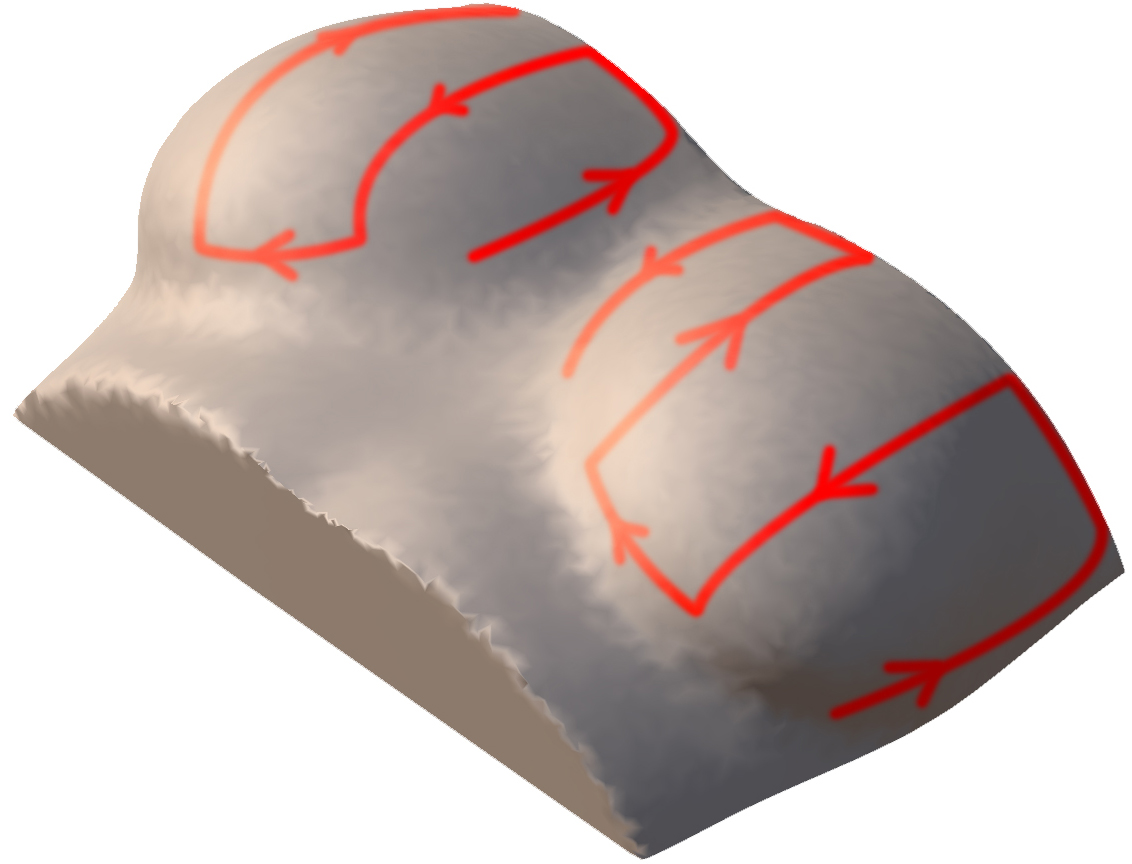
\includegraphics[width=0.75\textwidth]{figurer/d/probebevagelse}
    \caption{Ultralydsscannings bevægelsesmønster}
    \label{Probensbevagelse}
\end{figure}

Ifølge Lars Bolvig skal Automatisk Ultralydsscanner fungere ved, at radiografen tager videoklippene fra ultralydsscanningen og sender dem til radiologen, som vurderer videoklippene og det videre behandlingsforløb.

Se bilag \ref{Telefoninterview} Interview med radiolog Lars Bolvig for hele interviewet. 

\section{Økonomiske konsekvenser ved udvidelse af screeningsprogrammet} 
Der er udarbejdet en økonomisk analyse, da det er et væsentligt grundlag for indførsel af ny teknologi i sundhedssektoren. Analysen indeholder omkostningerne forbundet med implementering af Automatisk Ultralydsscanner, og hvilke økonomiske konsekvenser en udvidelse af screeningsprogrammet med ultralydscanninger vil have. Den økonomiske analyse er udført ved at lave et overslag over forskellen på udgifterne, hvis en radiolog skulle udføre ultralydsscanningerne, versus indførsel og implementering af Automatisk Ultralydsscanner. 

Analysen tager udgangspunkt i en break-even analyse.  Efter interview med radiolog Lars Bolvig blev det sandsynliggjort, at screeningsprogrammet kan udvides med ultralydsscanninger, hvor radiografer betjener Automatisk Ultralydsscanner. Det vil være samme procedure som ved mammografi, hvor radiologen gennemser røntgenbillederne. Break-even analysen undersøger, hvor mange ressourcer der kan flyttes fra en radiolog til en radiograf, ift. omkostningen relateret til implementeringen af Automatisk Ultralydsscanner, da en radiologs gennemsnitlige timeløn er 200 kroner højere end en radiografs \cite{Lon}.

Ifølge Lars Bolvig bruger radiologer meget tid på transport mellem arbejdsplads og scanningssted, f.eks. fra Aarhus til Holstebro, hvorfor transporttid er valgt som variabel. Se bilag \ref{Telefoninterview} Interview med radiolog Lars Bolvig. 

Samlede omkostninger for anskaffelse af udstyret til opsætning af Automatisk Ultralydsscanner er lavet på baggrund af antagelser, som f.eks. oplæring af radiografer, opsætning m.m. Tabellen \ref{FasteOmkostninger} nedenfor viser et skøn over udgifterne til indkøb, opsætning samt oplæring. Alle antagelser og udregninger kan ses i bilag \ref{Okonomi} Økonomisk analyse.

\begin{table}[htb]
\centering
\begin{tabular}{ | l | l | p{1\textwidth} | }
\hline
\textbf{Beskrivelse af udgift} & \textbf{DKK} \\\hline
Engangsudgifter til afskrivning & 201.668,00 \\\hline
Opsætning & 10.759,00 \\\hline
Oplæring af radiografer & 6.768,00 \\\hline
I alt & 219.305,64 \\\hline
\end{tabular}
\caption{Samlede udgifter for Automatisk Ultralydsscanner}
\label{FasteOmkostninger}
\end{table}

For begge scenarier er prisen for én ultralydsscanning beregnet, hvor tidsforbruget er antaget ud fra interview med radiolog Lars Bolvig og afdelingsradiograf Tine Bisgaard. Prisen pr. scanning med Automatisk Ultralydsscanner er udregnet ved at antage, at det er en radiograf, der foretager forberedelse, 3D scanning og betjener Robotarm under ultralydsscanning. En radiolog vil derefter bruge omkring 10 minutter på at tjekke scanningen igennem for at se, om patienten skal til en yderligere scanning. Prisen for én ultralydsscanning er beregnet til 110,64 kroner. 

Prisen for én ultralydsscanning ved scenariet, hvor en radiolog foretager ultralydsscanningen, er udregnet ved at antage, at det er en radiolog der står for både forberedelse og har en transporttid mellem arbejdsplads og scanningssted. Hvis transporttiden for radiologen er under fire minutter, er scenariet med Automatisk Ultralydsscanner dyrest. Tabel \ref{Breakeven} beskriver transportminutter og prisen for én ultralydsscanning udført af en radiolog. Den sidste kolonne beskriver antal scanninger, før Automatisk Ultralydsscanner er betalt hjem. Det vil sige, at der skal 35.052,51 ultralydsscanninger til, hvor radiologen har brugt fire minutter på transport, før Automatisk Ultralydsscanner er betalt hjem. Se bilag \ref{Okonomi} Økonomisk analyse for tidsestimeringer og yderligere beregninger. 

\begin{table}[H]
\centering
\begin{tabular}{ | c | c | c | p{0.49\textwidth} | }
\hline
\textbf{Transporttid (min.)} & \textbf{Pris pr. scanning (DKK)} & \textbf{Antal scanninger} \\\hline
5 & 116,89 & 35.052,51 \\\hline
8 & 135,34 & 8.873,09\\\hline
10 & 147,64 & 5.923,66\\\hline
15 & 178,39 & 3.235,19 \\\hline
20 & 209,14 & 2.225,25\\\hline
30 & 270,64 & 1.369,94\\\hline
45 & 362,89 & 868,95 \\\hline
60 & 455,14 & 636,26 \\\hline
\end{tabular}
\caption{Break-even analyse for antal transportminutter}
\label{Breakeven}
\end{table}

Analysen er et overslag og ikke en nøje udført business case, da alle udregninger er et skøn. Analysen ville fremstå bedre, hvis  flere radiologer havde medvirket til estimering af tider på ultralydsscanninger. Det er generelt forsøgt at prissætte udgifterne forbundet med indførslen af Automatisk Ultralydsscanner relativt højt for at undgå for mange uforudsete omkostninger. Hvis et hospital vil købe udstyret, vil priserne for opsætning måske være lavere, hvis man laver en indkøbsaftale. Beregningerne har ikke taget højde for, at radiologen udfører flere ultralydsscanninger for én transporttid. Transporttid må derfor ses som et gennemsnit pr. patient.

Som en del af screeningsprogrammet bliver der i Danmark udført omkring 270.000 mammografiundersøgelser \cite{esundhed}. Det betyder, at Automatisk Ultralydsscanner med en pris på 110,64 kroner pr. ultralydsscanning vil øge udgifterne til screeningsprogrammet med omkring 30 mio. kroner årligt. Yderligere vil omkostninger til indkøb og vedligeholdelse af Automatisk Ultralydsscanner medfølge. 

\section{Litteratursøgning om screeninger}
Det er undersøgt, hvilke andre konsekvenser en udvidelse af screeningsprogrammet for brystkræft vil medføre. Der er søgt med emneord inden for problemformuleringen i både national og international litteratur på de større databaser (PubMed, Cochrane etc.) for blandt andet at undersøge, om tidlig detektering af brystkræft er rentabel og omkostningseffektiv. 

Argumenter for at udføre screeninger er, at behandling af brystkræft på et tidligt stadie kan redde 6 ud af 1.000 kvinder fra at dø \cite{Argumenter}, og omkostninger til behandling stiger ved behandling på senere stadier \cite{StadieOmkostninger}. Et japansk randomized controlled trial (RCT) viste, at der ved kombinationen af ultralyds- og røntgenundersøgelser blev fundet flere stadium 0 og I kræft i interventionsgruppen, der både modtager ultralyds- og røntgenscanninger. Ved stadie II  var der ikke signifikant forskel \cite{Japan}. Det amerikanske Cancer Society har estimeret, at den relative overlevelsesprocent ved stadie 0 og I er tæt på 100\%, en overlevelsesprocent på 93\% ved stadie II, mens stadie III har en på 72\% og stadie IV har en overlevelsesprocent på 22\% \cite{CancerSociety}. Dette taler for at indføre ultralydsundersøgelser til screeningsprogrammet. 

Argumenterne imod er, at 13 ud af 1.000 kvinder vil blive udsat for overdiagnosticering, hvor patienter unødvendigt overbehandles, og at screeninger kan give patienten falsk tryghed \cite{Argumenter}. Det japanske RCT studie fandt, at der var en højere rate af falsk-positive tilfælde ved at anvende ultralyd sammen med mammografi \cite{Japan}. Et uafhængigt panel sammensat af Department of Epidemiology and Public Health, UK, undersøgte 11 RCT'er. Panelet estimerede, at ved screening for brystkræft af 10.000 50-årige kvinder, vil 43 brystkræftsrelaterede dødsfald blive forhindret, mens 129 vil blive overdiagnosticeret \cite{Panel}. Et Cochrane review undersøgte RCT's, der sammenlignede to grupper, hvor den ene screenes for brystkræft. Reviewet konkluderede, at screening reducerer brystkræft med 15\%, mens 30\% overdiagnosticeres og får behandling uden grund \cite{Gotzche}. Et BMC Cancer review undersøgte konsekvenserne af at lave en ultralydsscanning af brystet efter, en røntgenundersøgelse med et negativt resultat. Studiet fandt begrænset evidens for, at ultralyd er en fordel. Tre gange så mange kvinder fik lavet en biopsi ved ultralydsscanninger, hvor den positive prædiktive værdi gennemsnitlig er 10,3 \%. Det betyder flere falsk-positive prøver ved biopsier, mens den positive prædiktive værdi gennemsnitlig er 38\% ved mammografi \cite{DenseBreast}. 

Som pejlemærke til omkostningseffektiviteten kan man benytte kvalitetsjusterede leveår (QALY) til at beskrive, hvor rentabel en behandling er. I Danmark er der ikke en officiel grænse for, hvor meget én QALY bør koste, men Sundhedsstyrelsen (SST) har beskrevet: \textit{”...at man generelt anser behandlinger, der koster mindre end 160.000 kr. pr. QALY for omkostningseffektive, mens behandlinger der koster mere end 800.000 kr. pr. QALY anses for ikke at være omkostningseffektive”} \cite{QALY}. 
Et spansk studium undersøgte inkrementelle omkostninger ved henholdsvis ingen, årlige og biennale scanninger. Studiet viste, at gå fra ingen scanninger, til scanninger hvert andet år svarer til 4,469 € pr. QALY \cite{SpanskStudie}, 33.241,76 kr., hvilket er omkostningseffektivt efter SST's beskrivelse. National Health Service konkluderede i et RCT, at screeninger var forbundet med en ekstra omkostning på 45.5 mio. £ i det engelske sundhedsvæsen, svarende til 20.800 £, eller 183.335 kr., pr. vunden QALY \cite{NHS}.

Størstedelen af litteraturen konkluderer, at mere forskning er nødvendig på området. Det kan derfor være svært at lave en endelig konklusion på, hvorvidt en udvidelse af screeningsprogrammet vil være en god idé. Fordelen er, at man ved en kombination af ultralyd og røntgen kan opdage tidligere stadier af kræft, hvilket er billigere, og overlevelsesprocenten er højere. Ulemperne er, at der sker overdiagnosticering ved screeninger, og patienter derfor behandles uden grund. Tilføjelse af ultralydsscanninger til screeningsprogrammet vil øge omkostningerne og dermed prisen pr. QALY, hvilket sandsynligvis vil betyde, at udvidelse af screeningsprogrammet ikke er omkostningseffektivt. Se bilag \ref{Litteraturstudie} Litteraturstudie om screeninger, for hele analysen. 
